%!TEX root = ../../main.tex

preferably fungible

\chapter{Deployment}
This chapter is about the deployment step. Details about the backend are described first, then the API as an interface between the latter and the frontend gets explained and afterwards, the implementation of the frontend will be worked through.
\section{Backend}
Here, the overall architecture, structure, and functionality of the backend is explained. Afterwards, each of its components is described in detail. In the end, the installation and usage of the backend are shown.
\subsection{Overview}
The backend has the job to integrate several independent functionalities with each other and by that being able to serve the frontend.
As each of the functionalities is independent of the others, the main idea is to keep them modularized. This not only increases maintainability but also allows for independent development and testing of each module. These modules and their interactions with each other are shown in \autoref{fig:architecture_backend} and further described in the following.
\begin{figure}[H]
\centering
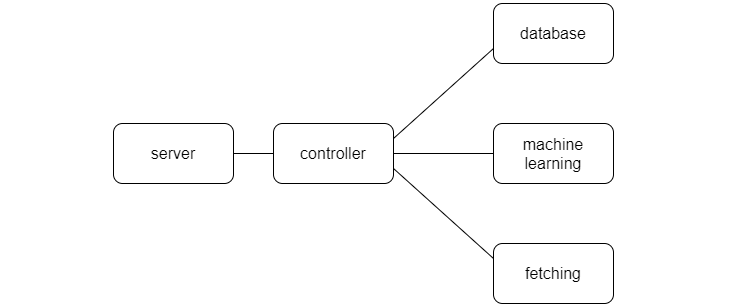
\includegraphics[width=1\textwidth]{images/modules.png}
\caption{Architecture of the backend}
\label{fig:architecture_backend}
\end{figure}

\subsection{Server}
The server module consists only of one equally named file and is the entry point of the backend. Its job is to hold a python-specific web server named 'flask'. The only thing except for the flask-part in this module is the access to the controller.
\newline
So in this file, every API-route is defined and for each route, an accordingly named function within the controller is called. The return value of it is then returned to the HTTP client, which sent the request.

\subsection{Controller}
Like the server module, the controller also consists of only one file. Yet it is the heart of the backend and orchestrates every action. The server requests answers from the controller according to the accessed route and the controller pulls all the triggers and data moving to create the desired answer. The file also contains all required global variables for every model - be it database-filename (more on that later) or model names. Therefore it is the single point of truth for backend variables. It contains one method for each route of the server plus on to predict a single match, as this requires playing together of the database and machine learning module.

To get a list of matches, be it with the results of classification or regression, a method from the database-module is called and before returning the list of matches, each match gets slightly modified. First, the date, which is stored as string in the database (due to the lack of a date-type in SQLite) is formatted to match the API-format (described in the next chapter). Afterwards, the actual result in the API-conform is created out of the two distinct goal-values.

Fetching new games and inserting them into the database requires a loop over all matches returned by the fetching module, preparing data for prediction, predict both the classification and regression result, and writing each match with all the values into the database. This ensures, that the database always contains predictions for each match.

Retraining the classification and regression model can be done independently, but the workflow is very similar. First, every match is retrieved from the database, then each match gets enriched by the additional data required for prediction, then the machine learning model receives this new list, executes the training, and returns the new model. The controller then again calls the machine learning module and saves the new model to disk. Afterwards, every match is repredicted and updated in the database.

\subsection{Database}
This module has its own folder because it requires several files. First of all, there is a python file, which contains all database-specific methods. Out of simplicity and experience, the chosen database-engine was SQLite, whose file is also stored in this folder. Each of the methods gets the filename of the database passed as an argument. They contain an enormous amount of really long comments, so future developers have it easier to understand not only the database schematic but also all of the data creation. There are functions for creating the database file (if it not already exists), add a new match to it, update either the prediction of classification or regression. While these were methods to add data to or update data in the database there are also three functions for getting data from the database. First, there is the option to get a single match, which is only used for testing purposes. Next comes a high-level function that returns the cumulated stats of the last ten matches of a specific team. It takes into account both playing as home team and as an away team. Last but not least there is a function to receive all matches in the database, sorted from newest to oldest. The file contains one additional helper method which is for retrieving data from the database as a type dictionary instead of an array for each entry.

\subsection{Fetching}
The fetching module also has its own folder, but it would not explicitly be required to have so. This is due to an earlier development time when the required data for fetching was downloaded as file and not directly into a variable. Later on, it was decided to leave it like this, as through the folder structure it gets clear, that database, fetching, and machine learning are quite different from the server and controller. The module contains only one function, which is for fetching a complete season. Which season it is, is announced by an argument placed by the controller. There are two data sources that have to be fetched, their results have to be merged together and then get returned to the controller. The first data source is a CSV-file which is downloaded from \url{http://www.football-data.co.uk/mmz4281//D1.csv} (\lstinline[columns=fixed]{} should match the desired season in the format of f.e. \lstinline[columns=fixed]{'19-20'}) and contains every finished match of the season with a lot of additional information needed for the machine learning part like odds, shots per team, etc.
The other datasource is the website \url{https://www.worldfootball.net/all_matches/bundesliga-20-20/} where \lstinline[columns=fixed]{} and \lstinline[columns=fixed]{} also equal to f.e. \lstinline[columns=fixed]{'19'} and \lstinline[columns=fixed]{'20'} respectively. This additional datasource is required to retrieve also upcoming matches which were not contained in the first datasource. Additionally, this second datasource contains a better readable teamname instead of abbreviations.
After both match lists are merged, the resulting, more complete list is returned back to the controller.

Currently, the upcoming matches are not added to the returned list. This is due to the fact, that machine learning requires f.e. the betting odds as input and this information is not freely available. %TODO

\subsection{Machine learning}
Like the two previous submodules, the machine learning module has its own folder. This is necessary because this module also contains the models for classification and regression. The single file with the multiple methods contains a simplified version of the same code used in the Jupyter notebooks for development, which is why they aren't explained in detail. Exceptions are a function to execute one of the two models on a match, a simplified retraining method and methods for the preparation of data for predictions. For the latter, the high-level function receives data for a specific match, which should be predicted and a list of the last 10 matches for each team. It then uses a lower-level function to calculate the total amounts of f.e. shots, shots on target, etc. and pulls together the calculated values to return to the controller. Because the classification-training requires slightly differently prepared data as the regression-training, there are two closely related but still independent methods for each of the data preparations.

\subsection{Installation and usage}
To run the backend python is required. The software was developed under version \lstinline[columns=fixed]{3.8.2} but should support the newer version as well. To install all of the dependencies, there is a file named \lstinline[columns=fixed]{requirements.txt} which contains all the additional software with their respective versions. To install them, simply run \lstinline[columns=fixed]{pip install -r requirements.txt}. To start the backend, just run \lstinline[columns=fixed]{py server.py} and wait until the message with the local port appears (approx. 2s).

\section{API}
As the back- \& frontend were developed independently, an API as an interface between them was developed. All of the below calls are HTTP GET methods.
\newline
\newline
In total there are two ways a call is answered by the backend. The first one is the return of a JSON-object, that the frontend has to process. The second one is a simple \lstinline[columns=fixed]{'ok'} string for actions that the backend has successfully finished. While the latter is self-explaining, the former had to be agreed upon for both front- and backend.

\subsection{/soccerGamesClassification}
As shown in \ref{lst:jsonsoccerGamesClassification}, this route returns a JSON-object named 'SoccerMatches' containing all soccer matches, with their respective dates, names of both teams, the predicted result and the actual result (if available). Each of those attributes is of type string. For the team names, this definitely makes sense, but as JSON lacks a type for a date, it was also chosen to be a string in the format of \lstinline[columns=fixed]{'DD/MM/YYYY'}. Again, both front and backend had to make sure to use the same formatting for this string. The predicted Result is actually a single character (Namely \lstinline[columns=fixed]{'D'} for draw, \lstinline[columns=fixed]{'H'} for home team win and \lstinline[columns=fixed]{'A'} for the away team win), but again, JSON doesn't have a dedicated type for it. For the actual result of the match, it would also be possible to create two integers, one goal-counter for each team, but this way the backend would just concatenate both numbers with a colon in between and pass this to the frontend.

\begin{lstlisting}[language=JSON,label={lst:jsonsoccerGamesClassification}, caption=JSON structure of API call on /soccerGamesClassification]
{
    "SoccerMatches": [
        {
            "date":<string>,
            "homeTeam":<string>,
            "awayTeam":<string>,
            "predictedResult":<string>,
            "actualResult":<string>
        },...
    ]
}
\end{lstlisting}

\subsection{/soccerGamesRegression}
This route returns the exact same JSON-object as the previous one and as already shown in \ref{lst:jsonsoccerGamesClassification}. The only difference is the field content of the predicted result: Instead of the previous single character, this time the string has the same format as the actual result with the structure of \lstinline[columns=fixed]{<predicted home team goals>:<predicted away team goals}.

\subsection{/retrainClassification}
As the backend is able to create a newly trained model, this feature has to be accessed from the frontend. It does so, by sending a GET request to this route and waiting for it to return 'ok'. When this happens, the backend has finished creating a new model to use for classification.

\subsection{/retrainRegression}
Closely related to the previous \lstinline[columns=fixed]{/retrainClassification} route, the only difference is the model, which is newly created by the backend; instead of the model for classification, this one overwrites the model used for regression.

\subsection{/fetchNewMatches}
With a GET call on this route, the backend is commanded to download a new list of matches, both historic and upcoming ones. After the download, it has to integrate them into the database for further usage.

After reading about all the routes, it could be argued, that there is no route for (re-) execution of the prediction for all matches in the database. This is possible due to the fact, that whenever the backend either fetches new matches or retrains a model, it (re-) executes both models on every match in the database. This may not be as efficient as a dedicated route for each model, but it is just as effective. Additionally, this prevents locks, as everything is running sequentially. One more reason is the inefficiency introduced by working through all matches in the database two times - once for each model.

\section{Frontend}
This section describes the techniques used for the design and implementation of the frontend.
\subsection{Overview}
The frontend is the conversion of the data served from the backend to a graphical interface,
through the use of HTML, CSS, and JavaScript, so that users can view and interact with that data.

The frontend is developed by using Vue.js as a JavaScript framework for building user interfaces.
Additionally Bootstrap 4 is used to ensure responsive web design. Responsive web design is an approach to make web pages render well on a variety of devices and windows or screen sizes \cite{responsive:2011}. 
Vue-Axios which is an HTTP client library to establish the connection is used with the backend based on HTTP requests. 

\subsection{Implementation}
Vue.js features architecture focuses on declarative rendering and component composition.

Vue components extend basic HTML elements to encapsulate reusable code \cite{vue:2020}.
At a high level, components are custom elements to which the Vue's compiler attaches behavior. 
In Vue, a component is essentially an instance of Vue with predefined options.
In the interface, SoccerGame.vue is used as a component that defines the implementation of the different attributes of a soccer game.

The frontend contains two pages: A result prediction and goal prediction pages. Each of them 
receives HTTP GET requests from the backend which contains the functionalites to be executed and the data to be displayed.

\subsection{Results prediction}

The results prediction page receives the JSON object from the Uniform Resource Identifier (URI) /soccerGamesClassification containing all soccer matches and the final results, as described in the previous part.
A Uniform Resource Identifier is a string of characters that unambiguously identifies a particular resource \cite{uri:2005}.
The matches data are displayed in an HTML table, as shown in the following figure.
This graphical interface also implements the URI /retrainClassification to be able to send a GET request by clicking on the Retrain button in order to retrain the model.

\begin{figure}[H]
    \centering
    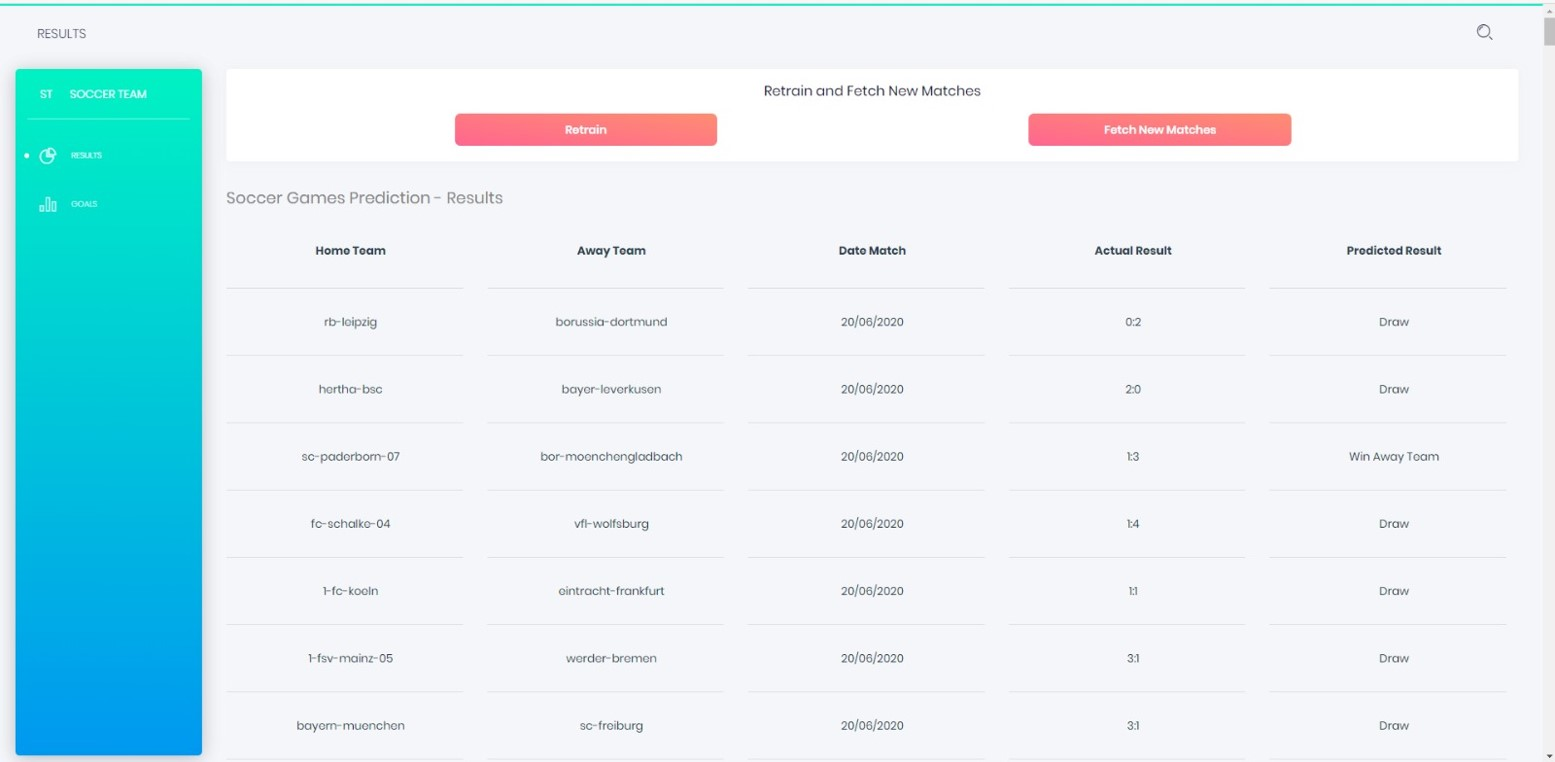
\includegraphics[width=1\textwidth]{images/frontend_results_prediction.jpg}
    \caption{The frontend webpage of the result prediction}
    \label{fig:result_frontend}
    \end{figure}

\subsection{Goals prediction}
This page implementation is very close to that of predicting results with few changes in the used URIs.
It receives the JSON object from the URI /soccerGamesRegression containing all soccer matches and the goals scored by each team.
It also implements the URI /retrainRegression to retrain the model. 
Both pages implement the same URI /fetchNewMatches functionality to download a new list of matches.
This functionality is performed by clicking on the Fetch New Matches button as shown in the following figure. 


\begin{figure}[H]
    \centering
    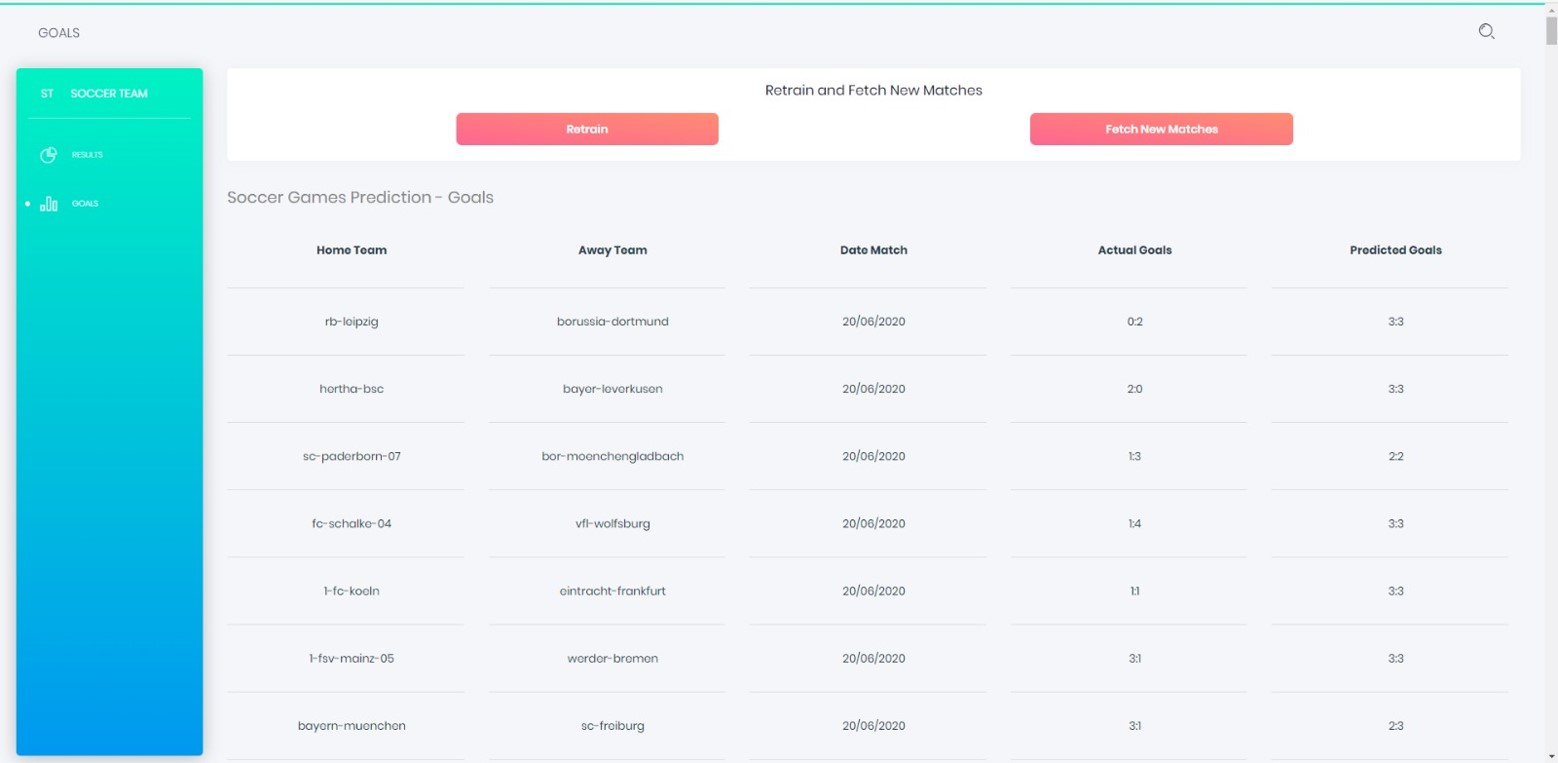
\includegraphics[width=1\textwidth]{images/frontend_goals_prediction.jpg}
    \caption{The frontend webpage of the goals prediction}
    \label{fig:goals_frontend}
    \end{figure}
